\section{Measurement with back-light illumination}
To measure the size and form of an object there are multiple ways. A popular way to get the contour is to place a light source behind the object desired to measure, and aim on the object with an camera. With this method the optical sensors get the silhouette of the object. In this section a short introduction to photometry and the typical construction of backlighting systems is discussed.
\subsection{Short introduction to photometry}
Photometry is the science concerned with the electromagnetic radiation visible to the human eye. In this section some important basics used further in this paper are explained. The theories of the following sections were taken from the textbook Physik 2 \cite{ruh}
\subsubsection{Photometric quantities}
In principle the normal physical quantities and units such as watts and joules could be used for the measurements of light radiation. However, in order to take into account the spectral sensitivity of the human eye, special photometric quantities and units are introduced.\\

\begin{table}[ht]
\centering
\begin{tabular}{ |p{6cm} p{2cm}|p{6cm} p{2cm}|  }
	\hline
	\multicolumn{2}{|c}{Quantity}&\multicolumn{2}{|c|}{Unit} \\
	\hline\hline
	\multicolumn{1}{|c}{Name}			& \multicolumn{1}{|c|}{Symbol}	& \multicolumn{1}{c}{Name}	& \multicolumn{1}{|c|}{Symbol}	\\

	\hline
	Luminous flux		& \multicolumn{1}{|c|}{$\Phi_v$}	& lumen		& \multicolumn{1}{|c|}{lm}\\
	Luminous intensity 	& \multicolumn{1}{|c|}{$I_v$} 		& candela	& \multicolumn{1}{|c|}{cd}\\
	Luminance			& \multicolumn{1}{|c|}{$L_v$}		& candela/$\text{m}^2$	& \multicolumn{1}{|c|}{cd/$m^2$}\\
	Illuminace 			& \multicolumn{1}{|c|}{$E_v$} 		& lux (=lumen/$\text{m}^2$) 	& \multicolumn{1}{|c|}{lx}\\

	\hline
\end{tabular}
\end{table}

\subsubsection{Light source}
To model a light source it is assumed that the source is a very small point which emits the light rays in all directions and is measured in luminous flux. The density of the light rays is reduced with the factor $\frac{1}{r^2}$ with $r$ being the distance. Luminous intensity of the light is proportional to the density of the rays. This behavior has to do with the fact that the surface area $A$ of a sphere
\begin{align*}
A=\int_{0}^{2 \pi} \int_{0}^{\pi} r^{2} \sin \theta d \theta d \varphi=4 \pi r^{2}
\end{align*}
grows squared with the distance from the center $r$.
\begin{align*}
A = 4\pi r^2
\end{align*}
\begin{figure}[ht]
	\centering
	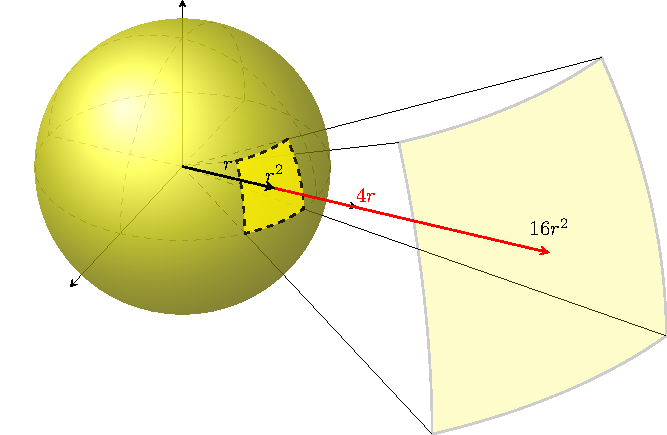
\includegraphics[width=0.6\textwidth]{2-theory/backlight/light.pdf}
	\caption{Light source in 3d\label{theory:light}}
\end{figure} 
\\
\subsubsection{Solid angle}
In photometry the usage of solid angle is very common. For the following the concept of solid angle must be defined. A beam of rays emanates from a point zero. The area that this beam illuminates on a sphere with center zero and radius 1 is called solid angle and is designated $\Omega$.
If spherical coordinates $r$,$\theta$ and $\varphi$ are used, a differential solid angle element $d \Omega$ can be expressed as followed
\begin{align*}
d \Omega=\sin \theta d \theta d \varphi
\end{align*}
The differential solid angle element can now be integrated to obtain a surface with $\hat{r}$ being the unit vector of the radius.
\begin{align*}
\Omega=\iint_{S} \frac{\hat{r} \cdot \hat{n} d S}{r^{2}}=\iint_{S} \sin \theta d \theta d \varphi
\end{align*}
When defining the solid angle, a sphere with any radius $r$ can be used instead of the unit sphere. The area A cut out by the beam of rays on the surface of the sphere must then be divided by $r^2$.
\begin{align*}
\Omega=\frac{A}{r^{2}}
\end{align*}
Solid angle is a dimensionless quantity.  

\subsubsection{Luminous flux}
Luminous flux or lumen is Luminous flux per unit time and has the unit candela steradians ($cd\cdot sr$). It is used to describe the total amount of light a lamp puts out and is named lumen (lm). To better understand how bright a lumen is there is a list with example values. \\


\begin{tabular}{ |p{12cm} p{2cm}|  }
		\hline
		& $\Phi_v$ in lm\\
		
		
		\hline
		LED		& 500\\
		Light bulb, 220 V, 60W		& 730\\
		Light bulb, 220 V, 100W		& 1'380\\
		Fluorescent tube, 220 V, 40W		& 2'300\\
		Mercury vapor lamp, 220 V, 125W		& 5'400\\
		Mercury vapor lamp, 220 V, 2000W		& 125'000\\
		\hline
\end{tabular}



\subsubsection{Luminous intensity}
Luminous intensity or candela is the Luminous flux per unit solid angle. It describes the perceived power per unit solid angle. As example we assume to have a light with a 10 lumen strong light source. If the light beam is now focused into 1 steradian light beam, the beam would be 10 candela.\\

\subsubsection{Luminance}
Luminace is the Luminous intensity per area of the luminous area
\begin{align*}
L_{\mathrm{v}}=\frac{\mathrm{d}^{2} \Phi_{\mathrm{v}}}{\mathrm{d} \Sigma \mathrm{d} \Omega_{\Sigma} \cos \theta_{\Sigma}}
\end{align*}\\

\begin{table}[ht]
	\centering
	\begin{tabular}{ |p{13cm} p{3cm}|  }
		\hline
		& $L_v$ in c/$\text{m}^2$\\
		
		
		\hline
		Fluorescent tube					& $10^4$\\
		Frosted light bulb					& $10^4...10^5$\\
		Tungsten filament of a light bulb	& $10^7...2\cdot 10^7$\\
		Arc lamp							& $1.5\cdot10^8...1.8\cdot10^8$\\
		High pressure mercury lamp			& $2.5\cdot10^8...10^9$\\
		Sun									& $1.2\cdot10^9$\\
		Xenon high pressure lamp			& $10^9...10^10$\\
		
		\hline
	\end{tabular}
\end{table}



\subsubsection{Illuminace }
\begin{table}[ht]
	\centering
	\begin{tabular}{ |p{12cm} p{3cm}|  }
		\hline
		& $E_v$ in lx\\
		
		
		\hline
		Sun light in summer					& 70'000\\
		Sun light in winter					& 5'500\\
		Day light with clouded sky			& 1'000-2'000\\
		Full moon night						& 0.25\\
		Stars without moon clear sky		& 0.001\\
		Limit of color perception			& 3\\
		Streetlight							& 1-30\\
		Living room							& 40-150\\
		Working room						& 40-300\\
		Working place lightning				& 100-4000\\
		
		\hline
	\end{tabular}
\end{table}




\begin{table}[ht]
	\centering
	\begin{tabular}{ |p{4cm} p{2cm} p{2cm}|p{4cm} p{2cm} p{2cm}|  }
		\hline
		\multicolumn{3}{|c}{Radiometry}&\multicolumn{3}{|c|}{Photometry} \\
		\hline\hline
		\multicolumn{1}{|l}{Name}			& \multicolumn{1}{c}{Symbol}& \multicolumn{1}{c|}{Unit}	& \multicolumn{1}{c}{Name}	& \multicolumn{1}{c}{Symbol}	& \multicolumn{1}{c|}{Unit}\\
		\hline
		Radiant flux			& \multicolumn{1}{|c|}{$\Phi_e$}&  \multicolumn{1}{|c|}{W}		& Luminous flux		& \multicolumn{1}{|c|}{$\Phi_v$}	&  \multicolumn{1}{|c|}{lm}\\
		Radiant intensity		& \multicolumn{1}{|c|}{$I_e$}	&  \multicolumn{1}{|c|}{W/sr}	&Luminous intensity 	& \multicolumn{1}{|c|}{$I_v$} 		&  \multicolumn{1}{|c|}{cd}\\
		Radiace					& \multicolumn{1}{|c|}{$L_e$}	&  \multicolumn{1}{|c|}{W/$m^2$sr}		&Luminance			& \multicolumn{1}{|c|}{$L_v$}		&  \multicolumn{1}{|c|}{cd/$m^2$}\\
		Irradiance flux density	& \multicolumn{1}{|c|}{$E_e$}	&  \multicolumn{1}{|c|}{W/$m^2$}		&Illuminace 			& \multicolumn{1}{|c|}{$E_v$} 		&  \multicolumn{1}{|c|}{lx}\\
		
		\hline
	\end{tabular}
\end{table}